\chapter{Implementacija i korisničko sučelje}
		
		
		\section{Korištene tehnologije i alati}
		
			Komunikacija u timu realizirana je korištenjem aplikacije WhatsApp\footnote{https://www.whatsapp.com/}. Za izradu UML dijagrama korišten je alat Astah Professional\footnote{https://astah.net/}, a kao sustav za upravljanje
			izvornim kodom Git\footnote{https://git-scm.com/}. Udaljeni repozitorij projekta je dostupan na web platformi GitLab\footnote{https://gitlab.com/}.\par
			
			Kao razvojno okruženje korišten je Intellij IDEA\footnote{https://www.jetbrains.com/idea/}
			- integrirano razvojno okruženje (IDE) tvrtke JetBrains\footnote{https://www.jetbrains.com/company/}. Prvenstveno se koristi za razvoj računalnih programa, kao i za web-stranice, web-aplikacije, i mobilne aplikacije. 
			Aplikacija je napisana koristeći radni okvir SpringBoot\footnote{https://spring.io/projects/spring-boot} i jezik Java\footnote{https://www.java.com/en/} za izradu backenda te React\footnote{https://reactjs.org/}
			i jezik JavaScript\footnote{https://www.javascript.com/} za izradu frontenda. React, takoder
			poznat kao React.js ili ReactJS, je biblioteka u JavaScriptu za izgradnju korisničkih sučelja. Održavana je od strane Facebooka\footnote{https://www.facebook.com/}. React se najčešće koristi kao osnova u razvoju web ili mobilnih aplikacija. Složene aplikacije u Reactu obično zahtijevaju korištenje dodatnih biblioteka za interakciju s API-jem. Spring\footnote{https://spring.io/projects/spring-framework} je široki skup biblioteka i alata koji olakšava razvoj aplikacija u Javi. Koristi anotacije, notacije i konvencije, koristeći oblikovne obrasce poput template-a i aspektno-orijentiranog programiranja.
			Jezgra Springa je tzv. inversion of control container ili aplikacijski kontekst, koji se temelji na oblikovnom obrascu koji se zove dependency injection.
			Koristili smo H2\footnote{https://www.h2database.com/html/main.html} bazu podataka na početku, a onda smo se prebacili perzistentnu Postgres\footnote{https://www.postgresql.org/} bazu.
		
	
		\section{Ispitivanje programskog rješenja}
			
			
			\subsection{Ispitivanje komponenti}
			Testirali smo 8 ispitnih slučajeva unoseći ispravne i neispravne podatke te provjeravajući vraća li sustav odgovore kakve očekujemo. Od osam ispitnih primjera, četiri se odnose na šetače te četiri na udruge. Rezultati i opisi pojedinih testova su priloženi ispod. Kao što ćemo vidjeti u rezultatima, svi su ispiti prolazni jer smo pri upisu neispravnih podataka i očekivali odgovore različite od 200 OK.
			
			\subsubsection{1. ispitni primjer - registracija udruge sa zauzetim OIB-om}
			
			U ispitnom primjeru prvo smo stvorili i registrirali prvu udrugu sa zadanim OIB-om 22000000000. Dobili smo očekivani odgovor sa statusom 200 OK. Zatim smo pokušali registrirati drugu udrugu sa istim tim OIB-om (ali drugačijim korisničkim imenom, koji također mora biti jedinstven). Dobili smo očekivani odgovor sa statusom 406 NOT ACCEPTABLE. Nakon toga smo promijenili OIB u 22000000001 te ponovno poslali zahtjev za registracijom. Dobili smo očekivani odgovor 200 OK.
			
			
			\begin{figure}[H]
				\centerline{
					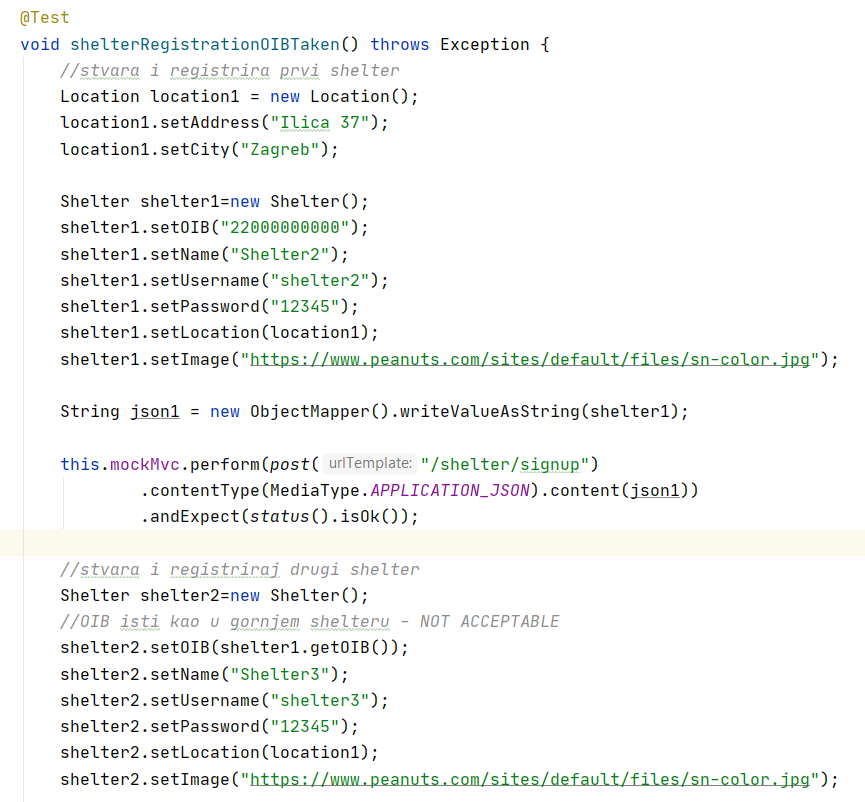
\includegraphics[scale=0.73]{slike/shelter1.1.PNG}}
				\hspace*{-0.21in}
				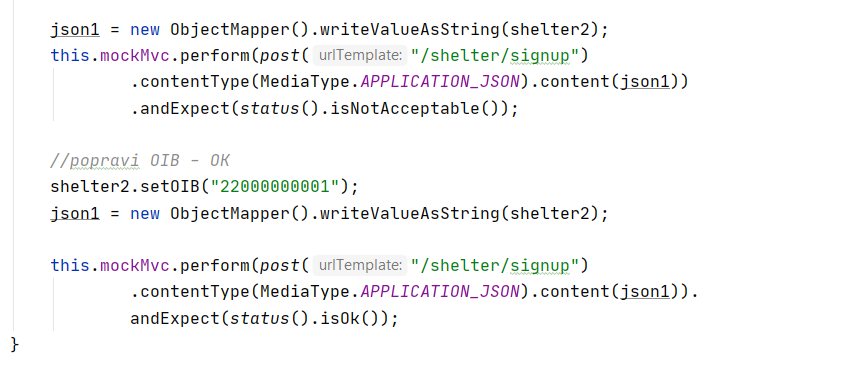
\includegraphics[scale=0.73]{slike/shelter1.2.PNG}
				%veličina slike u odnosu na originalnu datoteku i pozicija slike
				\centering
			\end{figure}
			
			
			
			\subsubsection{2. ispitni primjer - registracija udruge sa zauzetim korisničkim imenom}
			
			U ispitnom primjeru prvo smo stvorili i registrirali prvu udrugu sa zadanim korisničkim imenom "ella". Dobili smo očekivani odgovor sa statusom 200 OK. Zatim smo pokušali registrirati drugu udrugu sa istim tim korisničkim imenom (ali drugačijim OIB-om, koji također mora biti jedinstven). Dobili smo očekivani odgovor sa statusom 409 CONFLICT. Možemo primjetiti da je to drugačiji odgovor od onog u gornjem testu kada šaljemo OIB koji nije jedinstven (409 NOT ACCEPTED). To je zato što smo pomoću tih odgovora razlikovali kakav odgovor tj. feedback treba dati korisniku pri registraciji. Nakon toga smo promijenili korisničko ime u "lily" te ponovno poslali zahtjev za registracijom. Dobili smo očekivani odgovor 200 OK.
			
			\begin{figure}[H]
				\centerline{
					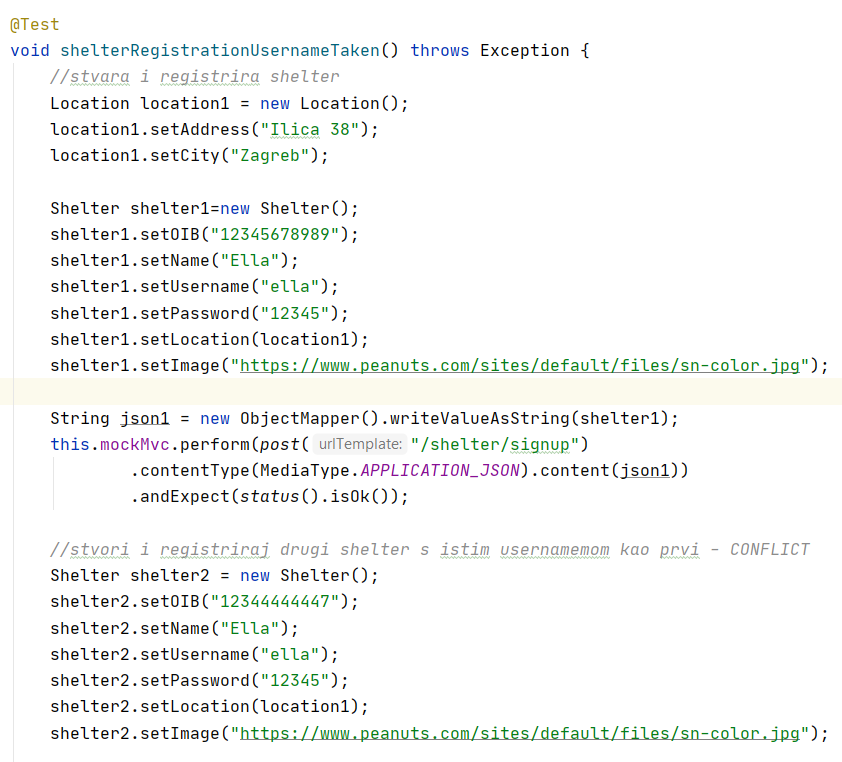
\includegraphics[scale=0.75]{slike/shelter2.1.PNG}}
				\hspace*{-0.22in}
				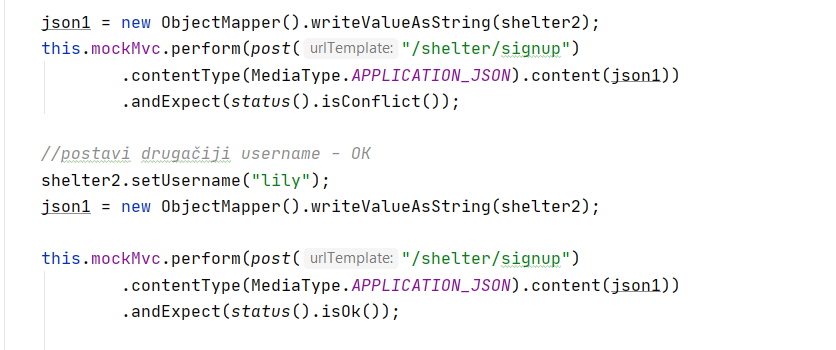
\includegraphics[scale=0.75]{slike/shelter2.2.PNG} %veličina slike u odnosu na originalnu datoteku i pozicija slike
				\centering
			\end{figure}
			
			
			
			\subsubsection{3. ispitni primjer - mijenjanje podataka udruge sa i bez autorizacije }
			
			U ispitnom primjeru prvo smo stvorili i registrirali  udrugu. Dobili smo očekivani odgovor sa statusom 200 OK. Također, u tijelu odgovora nam je vraćena ta udruga koju smo upravo registrirali uz dodatak ID-a udruge koji je stvoren na backendu. Taj vraćeni objekt smo spremili u našu varijablu udruge jer ćemo koristiti vraćeni ID u putanji za mijenjanje podataka. Zatim smo promijenili ime udruge u "NovoIme" te poslali zahtjev za promjenom. Dobili smo očekivani odgovor sa statusom 401 UNAUTHORIZED jer nismo dodali autorizaciju na zahtjev. Nakon toga smo pokušali ponovno sa dodanom autorizacijom te dobili očekivani odgovor 200 OK te udrugu sa promijenjenim imenom u tijelu odgovora. Na kraju smo provjerili da je u vraćenoj udruzi stvarno promijenjeno ime.
			
			\begin{figure}[H]
				\hspace*{-0.5in}
				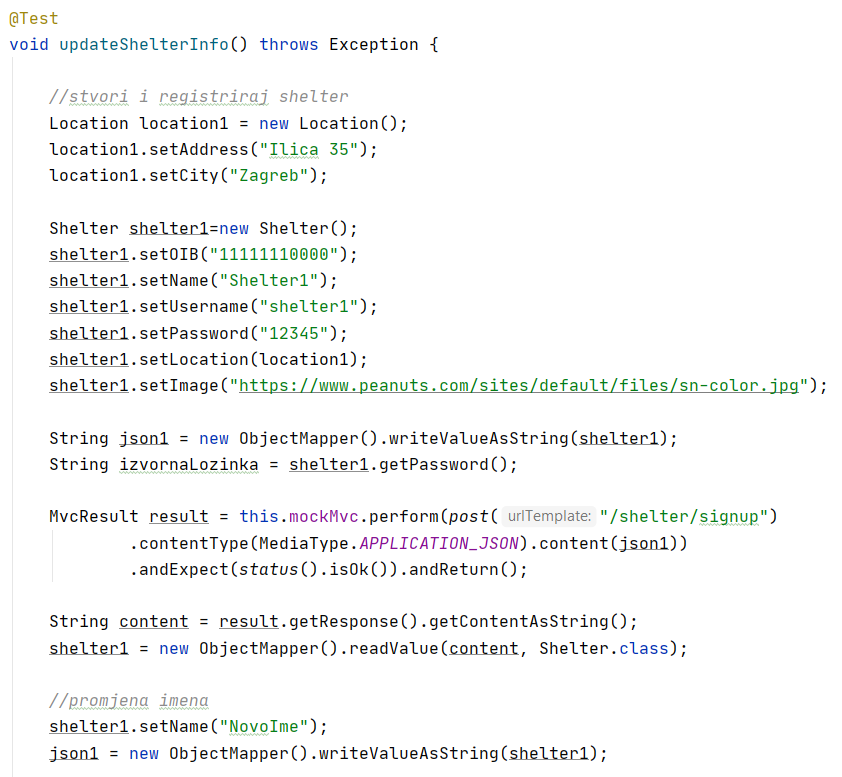
\includegraphics[scale=0.73]{slike/shelter3.1.PNG}
				\hspace*{-0.45in}	
				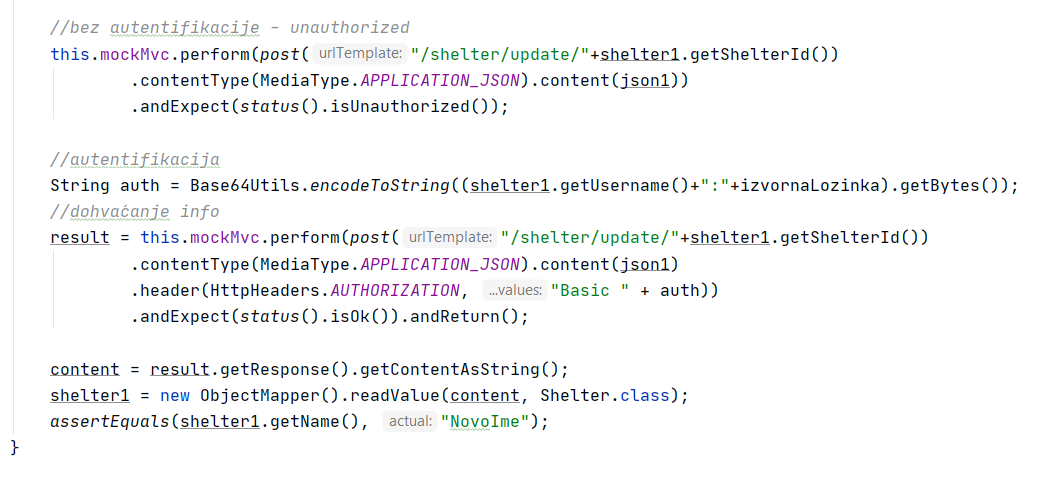
\includegraphics[scale=0.73]{slike/shelter3.2.PNG} %veličina slike u odnosu na originalnu datoteku i pozicija slike
				\centering
			\end{figure}
			
			
			\subsubsection{4. ispitni primjer - brisanje udruge sa i bez autorizacije }
			
			U ispitnom primjeru prvo smo stvorili i registrirali  udrugu. Dobili smo očekivani odgovor sa statusom 200 OK. Također, u tijelu odgovora nam je vraćena ta udruga koju smo upravo registrirali uz dodatak ID-a udruge koji je stvoren na backendu. Taj vraćeni objekt smo spremili u našu varijablu udruge jer ćemo koristiti vraćeni ID u putanji za brisanje udruge. Zatim smo poslali zahtjev za brisanjem bez autorizacije. Dobili smo očekivani odgovor sa statusom 401 UNAUTHORIZED jer nismo dodali autorizaciju na zahtjev. Nakon toga smo pokušali ponovno sa dodanom autorizacijom te dobili očekivani odgovor 200 OK.
			
			\begin{figure}[H]
				\hspace*{-0.93in}
				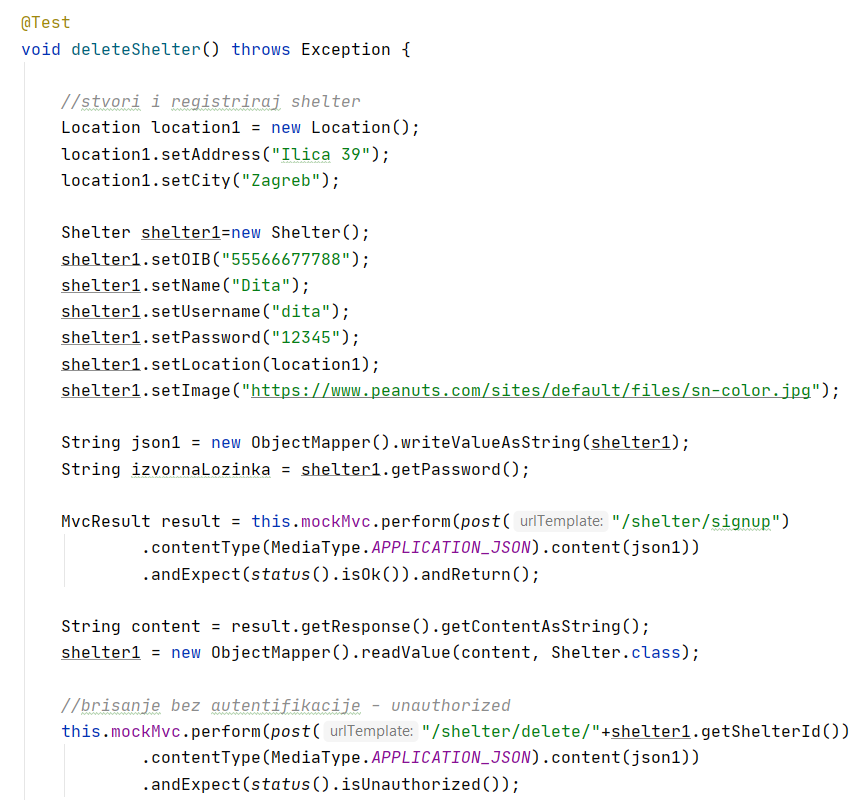
\includegraphics[scale=0.71]{slike/shelter4.1.PNG}
				\hspace*{-0.6in}
				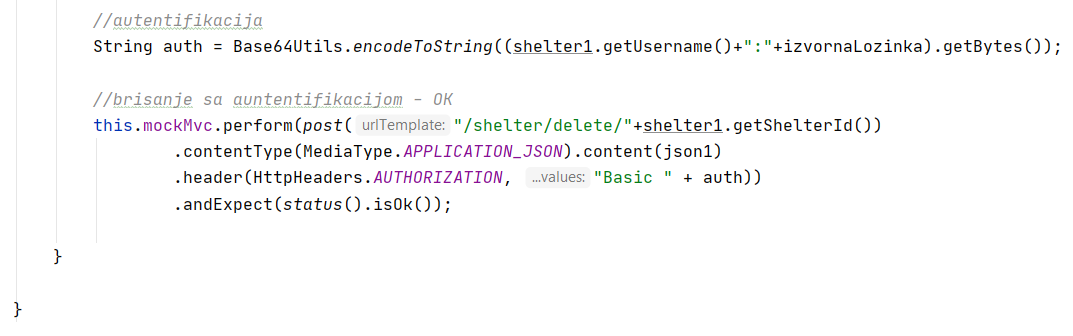
\includegraphics[scale=0.71]{slike/shelter4.2.PNG} %veličina slike u odnosu na originalnu datoteku i pozicija slike
				\centering
			\end{figure}
			
			
			
			\subsubsection{5. ispitni primjer - registracija šetača sa zauzetom email adresom}
			
			U ispitnom primjeru prvo smo stvorili dva šetača sa jednakim email adresama (ali različitim korisničkim imenima, koja također moraju biti jedinstvena). Registrirali smo prvog i dobili očekivani odgovor sa statusom 200 OK. Zatim smo pokušali registrirati drugog šetača te smo dobili  očekivani odgovor sa statusom 406 NOT ACCEPTABLE jer email adresa šetača mora biti jedinstvena.
			
			
			\begin{figure}[H]
				\centerline{
					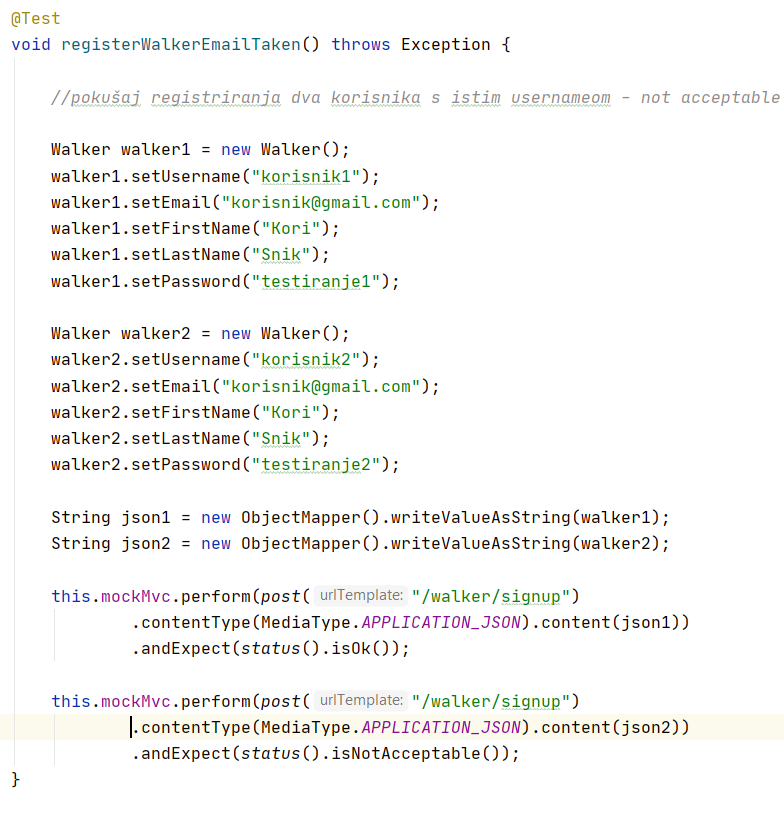
\includegraphics[scale=0.75]{slike/walker1.PNG}}
				%veličina slike u odnosu na originalnu datoteku i pozicija slike
				\centering
			\end{figure}
			
			\newpage
				
			\subsubsection{6. ispitni primjer - registracija šetača sa zauzetim korisničkim imenom}
			
			U ispitnom primjeru prvo smo stvorili dva šetača sa jednakim korisničkim imenom (ali različitim email adresama, koje također moraju biti jedinstvene). Registrirali smo prvog i dobili očekivani odgovor sa statusom 200 OK. Zatim smo pokušali registrirati drugog šetača te smo dobili  očekivani odgovor sa statusom 409 CONFLICT jer e korisničko ime šetača mora biti jedinstveno. Kao i u primjeru s udrugama, šaljemo različite statuse ovisno je li došlo do pogreške zbog korisničkog imena ili lozinke jer tako znamo kakvu poruku poslati korisniku.
			
			
			\begin{figure}[H]
				\centerline{
					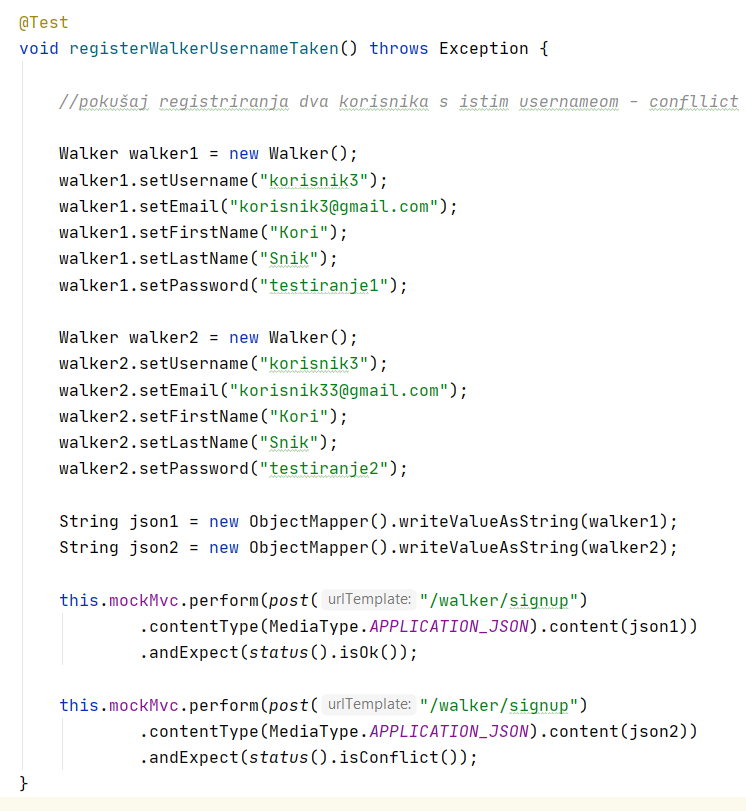
\includegraphics[scale=0.75]{slike/walker2.PNG}} %veličina slike u odnosu na originalnu datoteku i pozicija slike
				\centering
			\end{figure}
			
			
			\subsubsection{7. ispitni primjer - mijenjanje podataka šetača sa i bez autorizacije }
			
			U ispitnom primjeru prvo smo stvorili i registrirali  šetača. Dobili smo očekivani odgovor sa statusom 200 OK. Također, u tijelu odgovora nam je vraćen taj šetač kojeg smo upravo registrirali uz dodatak ID-a šetača koji je stvoren na backendu. Taj vraćeni objekt smo spremili u našu varijablu šetača jer ćemo koristiti vraćeni ID u putanji za mijenjanje podataka. Zatim smo promijenili korisničko ime šetača u "noviKorisnik" te poslali zahtjev za promjenom. Dobili smo očekivani odgovor sa statusom 401 UNAUTHORIZED jer nismo dodali autorizaciju na zahtjev. Nakon toga smo pokušali ponovno sa dodanom autorizacijom te dobili očekivani odgovor 200 OK te šetača sa promijenjenim korisničkim imenom u tijelu odgovora. Na kraju smo provjerili da je vraćenom šetaču stvarno promijenjeno ime.
			
			
			
			\begin{figure}[H]
				\hspace*{-0.58in}
				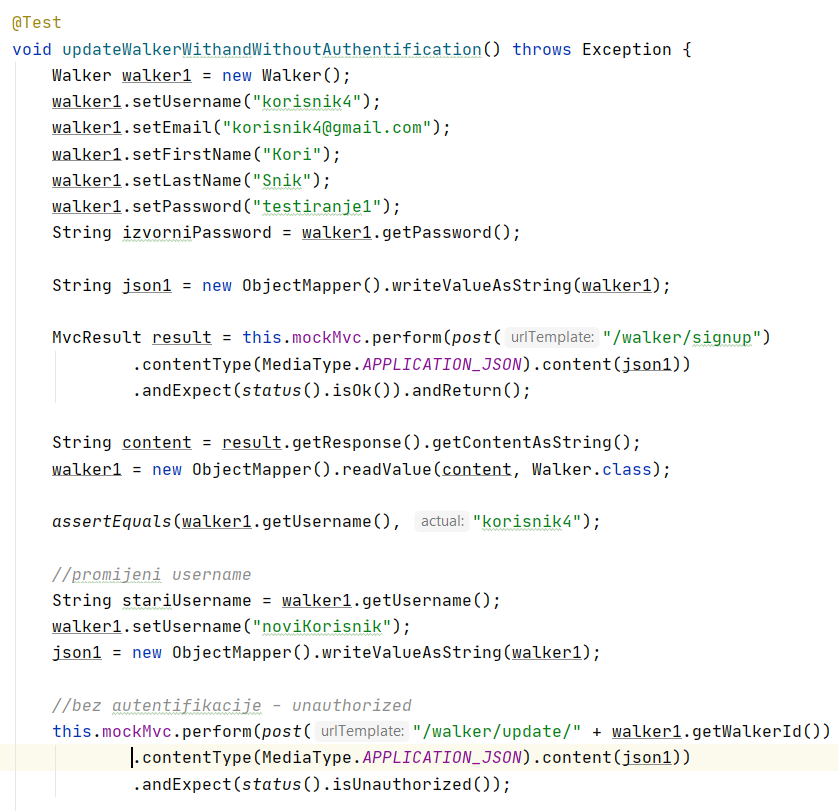
\includegraphics[scale=0.73]{slike/walker3.1.PNG}
				\hspace*{-0.41in}
				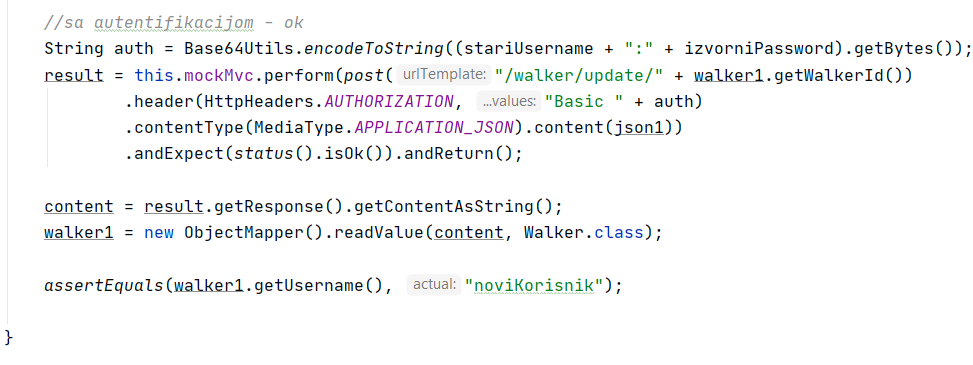
\includegraphics[scale=0.73]{slike/walker3.2.PNG} %veličina slike u odnosu na originalnu datoteku i pozicija slike
				\centering
			\end{figure}
			
			
			\subsubsection{8. ispitni primjer - mijenjanje podataka šetača sa i bez autorizacije }
			
			U ispitnom primjeru prvo smo stvorili i registrirali  šetača. Dobili smo očekivani odgovor sa statusom 200 OK.  Zatim smo stvorili novu šetnju te poslali zahtjev za rezervacijom šetnje (odabrali smo psa sa ID-jem 13 i stavili 13 u stazu "/reserve/13"). Dobili smo očekivani odgovor sa statusom 401 UNAUTHORIZED jer nismo dodali autorizaciju na zahtjev. Nakon toga smo pokušali ponovno sa dodanom autorizacijom te dobili očekivani odgovor 200 OK. 
			
			
			\begin{figure}[H]
				\hspace*{-0.18in}
				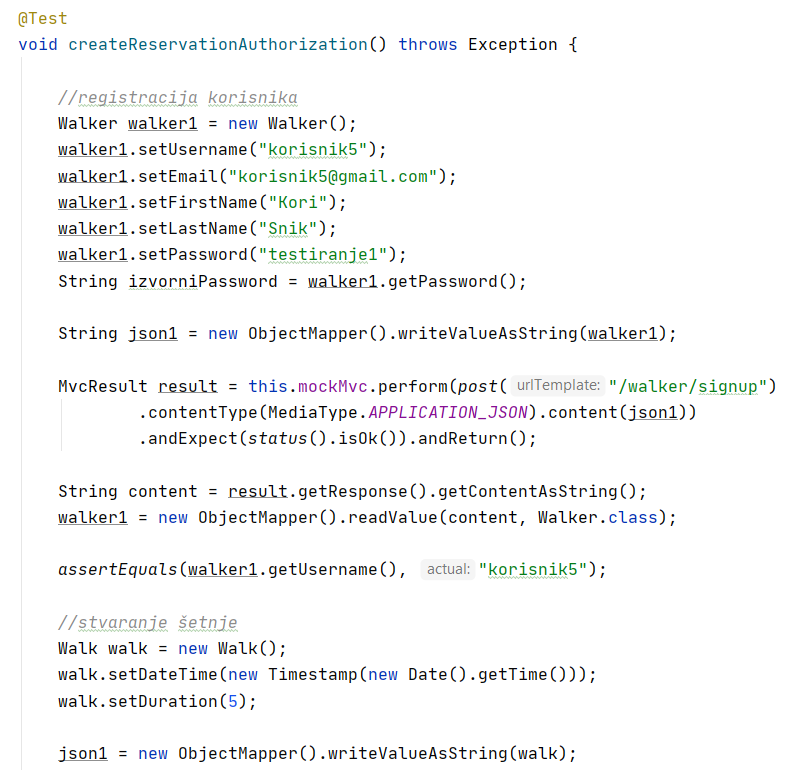
\includegraphics[scale=0.75]{slike/walker4.1.PNG}
				\hspace*{-0.4in}
				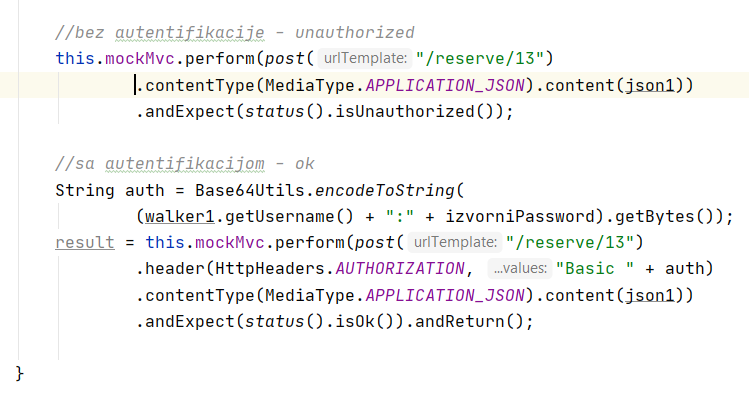
\includegraphics[scale=0.75]{slike/walker4.2.PNG} %veličina slike u odnosu na originalnu datoteku i pozicija slike
				\centering
			\end{figure}
		
		
			\subsubsection{Rezultati izvođenja ispitnih primjera }
			
			\begin{figure}[H]
				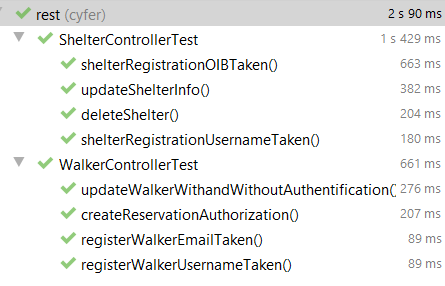
\includegraphics[scale=0.75]{slike/UnitRezultati.PNG}
				\centering
			\end{figure}
			
			\newpage	
			
			
			\subsection{Ispitivanje sustava}
			
				Za ispitivanje sustava koristili smo radni okvir Selenium. Uz podršku Selenium WebDrivera, napisali smo četiri ispita u programskom jeziku Java. Kao i u gornjim primjerima, svi ispiti su uspješno prošli jer smo pri slanju krivih podataka očekivali da su korisniku prikazane informacije o tome što je krivo. Svi ispiti su vezani uz varijacije registracija šetača i udruge. Očekivali smo da sustav zna reći koji podaci su neispravni kako bi ih mogao ispraviti.
			
			\subsubsection{1. ispitni primjer - registracija šetača sa ispravnim podatcima}
			
				U ovom primjeru smo demonstrirali uspješnu registraciju šetača. Upisali smo sve ispravne podatke - jedinstvenu email adresu i korisničko ime te lozinke koje se podudaraju. Od sustava smo očekivali da nas onda preusmjeri na početnu stranicu, što je ispunjeno.
				
				\begin{figure}[H]
					\hspace*{0in}
					
\includegraphics[scale=0.5]{slike/HomePage.PNG}
					\caption{Ispitni primjer 1 - Početna stranica}
					%veličina slike u odnosu na originalnu datoteku i pozicija slike
					\centering
				\end{figure}
				
			 	\begin{figure}[H]
			 	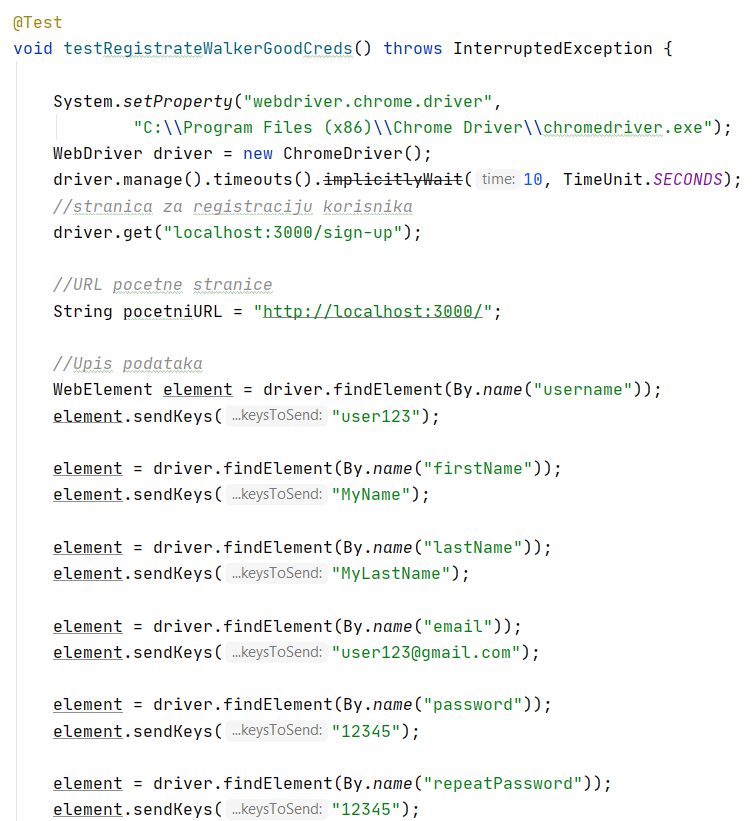
\includegraphics[scale=0.75]{slike/Selenium1.1.PNG}
			 	\hspace*{-0.85in}
			 	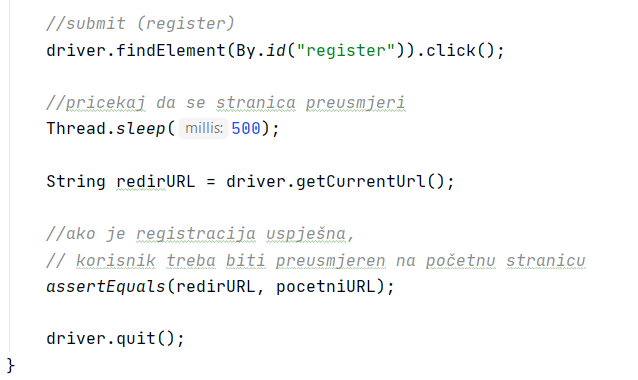
\includegraphics[scale=0.75]{slike/Selenium1.2.PNG} %veličina slike u odnosu na originalnu datoteku i pozicija slike
			 	\centering
			 \end{figure}
		 
		 
		 
		 \subsubsection{2. ispitni primjer - registracija šetača s neispravnim podatcima}
		 
		 U ovom primjeru smo demonstrirali neuspješnu registraciju šetača. Upisali smo isto korisničko ime kao i u gornjem primjeru - "user123", a kako smo ispite pokretali slijedno, takav korisnik je već bio u bazi. Od sustava smo očekivali da nam javi kakva je pogreška u pitanju. Sustav je ostao na istoj stranici (nije se dogodilo preusmjeravanje kao pri uspješnoj registraciji) te nam je ispisao poruku "Neuspješna registracija - korisničko ime je zauzeto." U ispitnom primjeru smo provjerili je li doista ispisana ta poruka. Ispod je priložena slika izvođenja u browseru te kod ispitnog primjera. 
		 
		 	\begin{figure}[H]
		 		\centerline{
		 		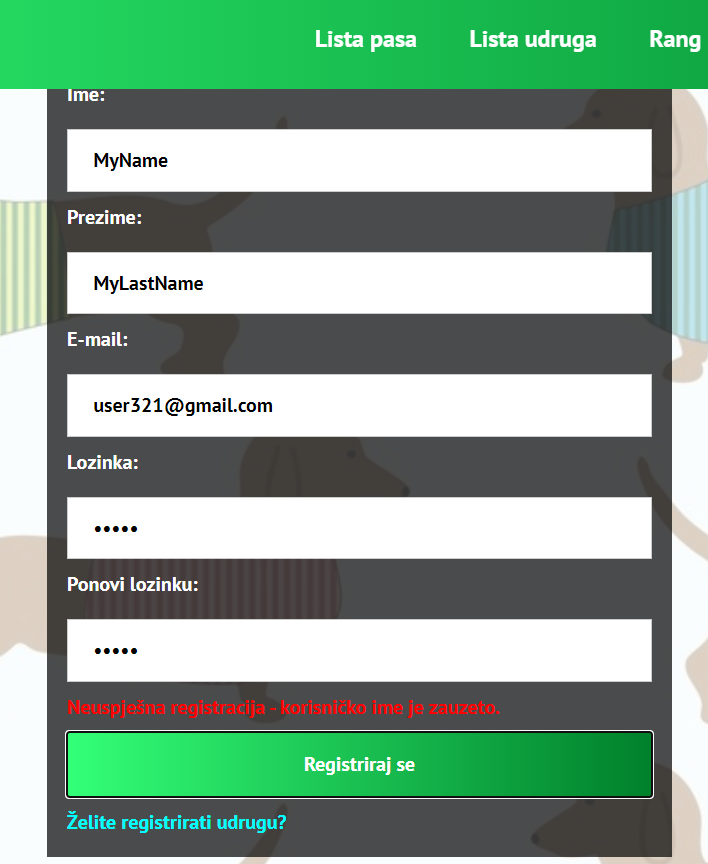
\includegraphics[scale=0.65]{slike/UsernameError.PNG}}
		 		\caption{Ispitni primjer 2 - Korisničko ime zauzeto}
		 		 %veličina slike u odnosu na originalnu datoteku i pozicija slike
		 		\centering
		 	\end{figure}
			 
			 \begin{figure}[H]
			 	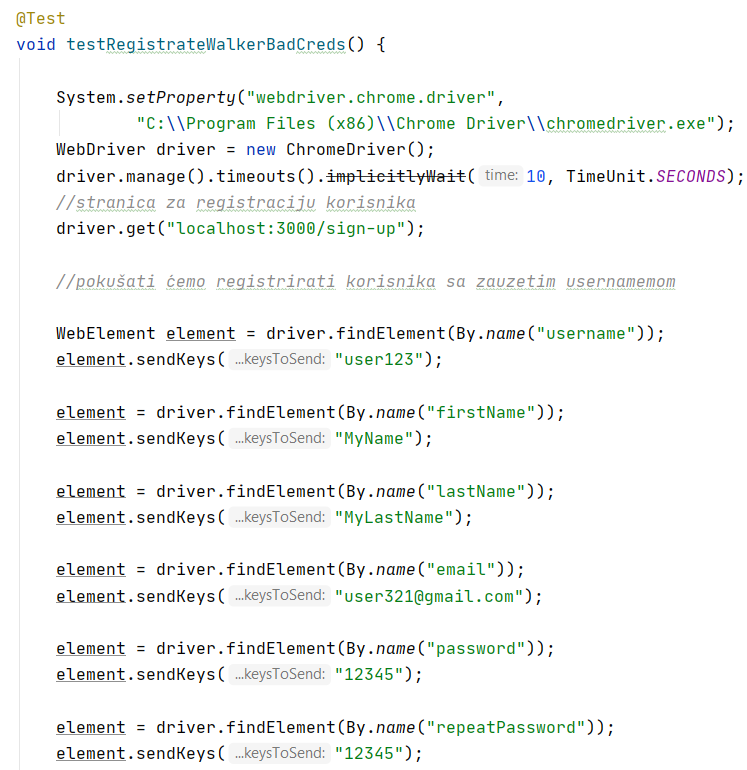
\includegraphics[scale=0.75]{slike/Selenium2.1.PNG}
			 	\hspace*{0.15in}
			 	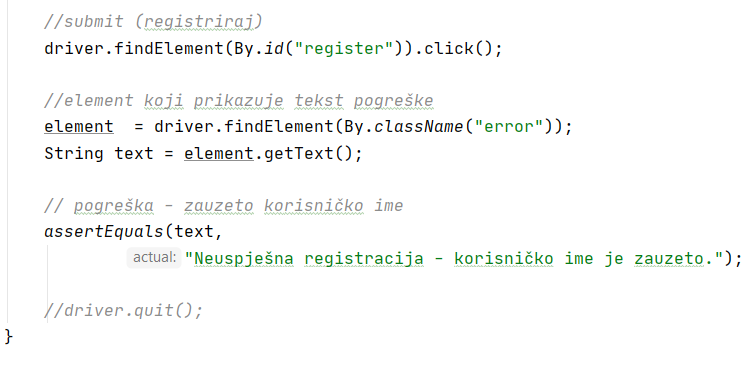
\includegraphics[scale=0.75]{slike/Selenium2.2.PNG}
			 	\caption{Ispitni primjer 2 - registracija šetača s neispravnim podatcima} %veličina slike u odnosu na originalnu datoteku i pozicija slike
			 	\centering
			 \end{figure}
		 
		 
		   \subsubsection{3. ispitni primjer - registracija udruge sa ispravnim podatcima}
		 
		 U ovom primjeru smo demonstrirali uspješnu registraciju udruge uz ispravak lozinke. Upisali smo sve ispravne podatke osim lozinke i ponovljene lozinke, koje su bile različite. Od sustava smo očekivali da nam javi kakva je pogreška u pitanju. Sustav je ostao na istoj stranici (nije se dogodilo preusmjeravanje kao pri uspješnoj registraciji) te nam je ispisao poruku "Lozinke se ne poklapaju." Zatim smo ispravili ponovljenu lozinku i ponovno poslali zahtjev za registracijom. Sustav nas je očekivano preusmjerio na početnu stranicu. Ispod je priložena slika izvođenja u browseru (neispravne lozinke) te kod ispitnog primjera. 
			 
			  \begin{figure}[H]
			  	\centerline{
			 	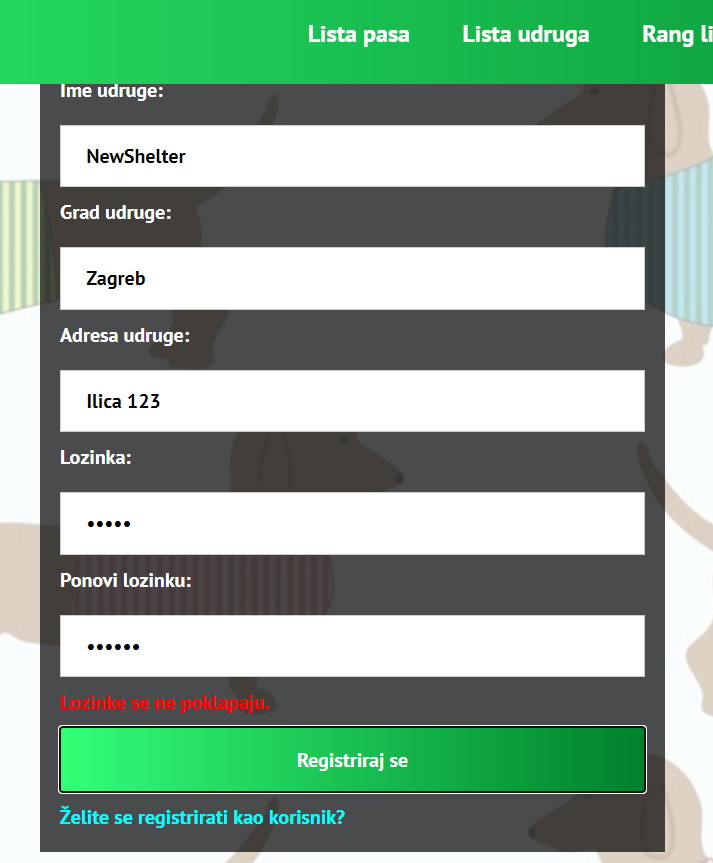
\includegraphics[scale=0.65]{slike/PasswordError.PNG}}
			 	%veličina slike u odnosu na originalnu datoteku i pozicija slike
			 	\caption{3. ispitni primjer - Nepodudaranje lozinka}
			 	\centering
			 \end{figure}
			 \begin{figure}[H]
			 	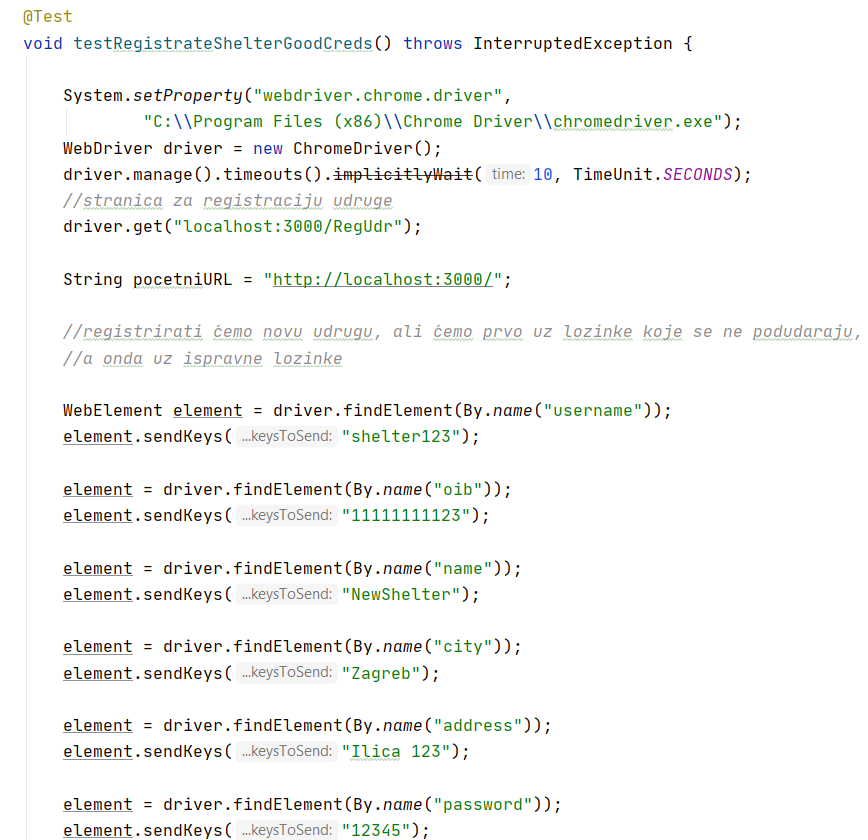
\includegraphics[scale=0.75]{slike/Selenium3.1.PNG}
			 	%veličina slike u odnosu na originalnu datoteku i pozicija slike
			 	\centering
			 \end{figure}
		 
			 \begin{figure}[H]
			 	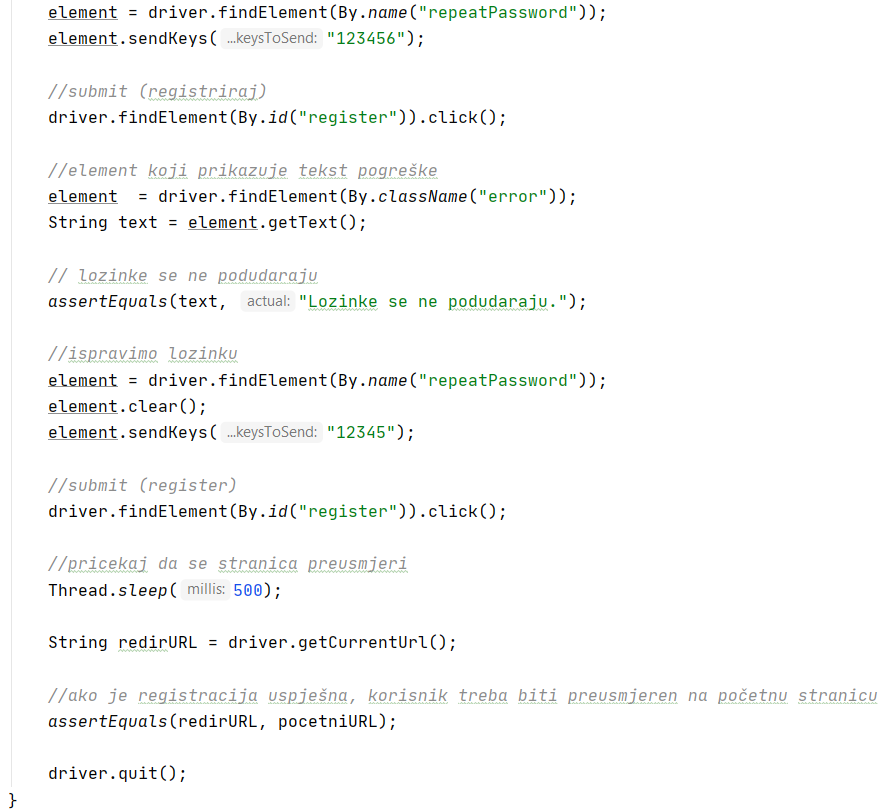
\includegraphics[scale=0.75]{slike/Selenium3.2.PNG} %veličina slike u odnosu na originalnu datoteku i pozicija slike
			 	\caption{Ispitni primjer 3 - registracija udruge sa ispravnim podatcima}
			 	\centering
			 \end{figure}
			 
			 \newpage
			 
			  \subsubsection{4. ispitni primjer - registracija udruge s neispravnim podatcima}
			 
			 U ovom primjeru smo demonstrirali neuspješnu registraciju udruge. Upisali smo isti OIB kao i u gornjem (trećem) primjeru - "11111111123", a kako smo ispite pokretali slijedno, takva udruga je već bila u bazi. Od sustava smo očekivali da nam javi kakva je pogreška u pitanju. Sustav je ostao na istoj stranici (nije se dogodilo preusmjeravanje kao pri uspješnoj registraciji) te nam je ispisao poruku "Neuspješna registracija - postoji već udruga sa danim OIB-om." U ispitnom primjeru smo provjerili je li doista ispisana ta poruka. Ispod je priložena slika izvođenja u browseru te kod ispitnog primjera. 
			 
			 \begin{figure}[H]
			 	\centerline{
			 	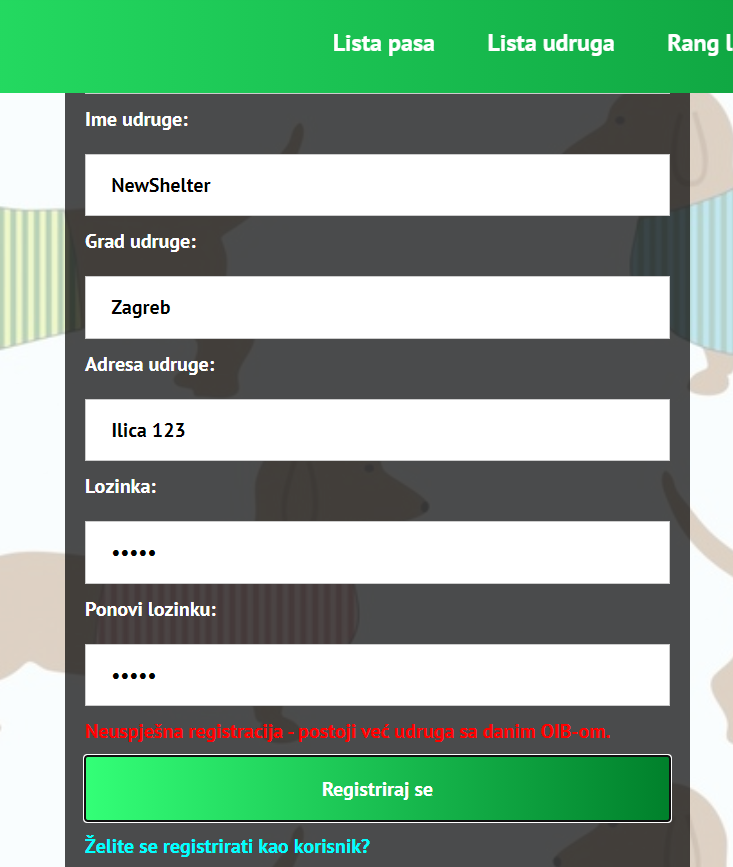
\includegraphics[scale=0.65]{slike/OIBError.PNG}}
			 	%veličina slike u odnosu na originalnu datoteku i pozicija slike
			 	\caption{Registracija udruge sa zauzetim OIB-om}
			 	\label{fig:wrongOIB}
			 	\centering
			 \end{figure}
			 \begin{figure}[H]
			 	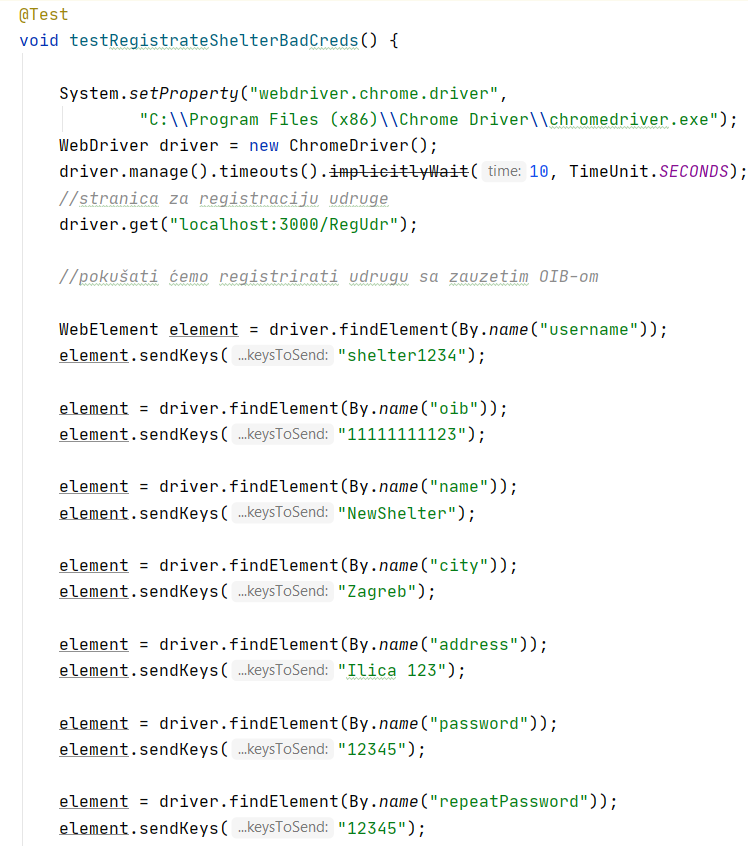
\includegraphics[scale=0.7]{slike/Selenium4.1.PNG}
			 	\hspace*{0.1in}
			 	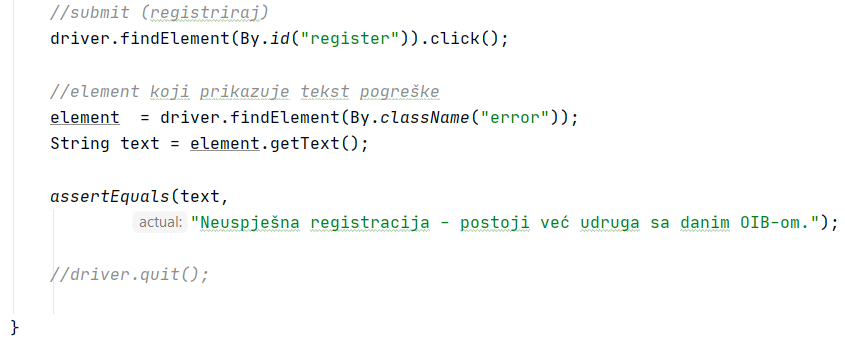
\includegraphics[scale=0.7]{slike/Selenium4.2.PNG} %veličina slike u odnosu na originalnu datoteku i pozicija slike
				\caption{Ispitni primjer 4 - registracija udruge s neispravnim podatcima}
			 	\centering
			 \end{figure}
		 
		 
		 \subsubsection{Rezultati izvođenja ispitnih primjera}
		 	\begin{figure}[H]
		 		\centerline{
		 		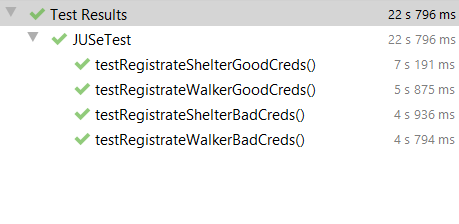
\includegraphics[scale=0.75]{slike/SeleniumRezultati.PNG}} %veličina slike u odnosu na originalnu datoteku i pozicija slike
		 		\caption{Rezultati izvođenja ispitnih primjera - Selenium}
		 		\centering
		 	\end{figure}
		 
		 
			
			\eject 
		
		
		\section{Dijagram razmještaja}
			
			%\textbf{\textit{dio 2. revizije}}
			
			% \textit{Potrebno je umetnuti \textbf{specifikacijski} dijagram razmještaja i opisati ga. Moguće je umjesto specifikacijskog dijagrama razmještaja umetnuti dijagram razmještaja instanci, pod uvjetom da taj dijagram bolje opisuje neki važniji dio sustava.}
			
			 Topologija našeg projekta sastoji se od dva čvora, od kojih su oba uređaji. Jedan je korisničko računalo, drugi je poslužiteljsko računalo. Na poslužiteljskom računalu nalaze se svi potrebni izvorni kodovi i baza podataka kako bi se ostvario uspješan deploy web aplikacije. Programska potpora sastoji se od kombinacije Spring frameworka i ReactJs-a. Također, korisničko i poslužiteljsko računalo međusobno razmjenjuju informacije putem HTTP protokola.
			
			~\\
			\begin{figure}[H]
				\hspace{-0.4in}
				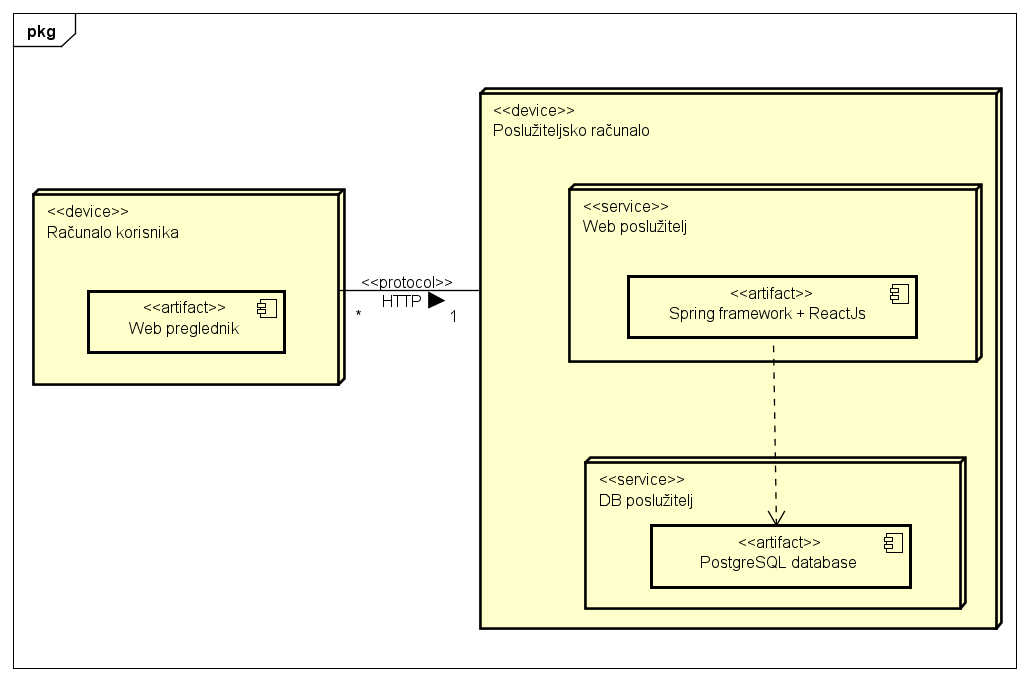
\includegraphics[scale=0.65]{dijagrami/Dijagram razmjestaja.png} %veličina slike u odnosu na originalnu datoteku i pozicija slike
				\caption{Dijagram razmještaja}
				\centering
			\end{figure}
			
			
			\eject 
		
		\section{Upute za puštanje u pogon}
		
		Puštanje aplikacije u pogon (engl. deploy) proces je na kraju kojega aplikacija koju smo prethodno pokretali s našeg lokalnog poslužitelja (engl. localhost) postaje javno dostupna na internetu. Kao cloud platformu za deploy odabrali smo Heroku, na koji smo kao odvojene aplikacije postavili frontend i backend. Na backend aplikaciji smo podesili PostgreSQL bazu koja se isto tako nalazi na Heroku. Na kraju smo povezali frontend i backend aplikacije putem proxyja tako da su na jednom mjestu dostupne sve funkcionalnosti.
		Frontend i backend smo deployali kao odvojene aplikacije jer imamo monorepozitorij na GitLabu, što bi nam otežalo proces puštanja u pogon da smo se odlučili za opciju deploya preko gita.\par
		
		\subsection{Puštanje u pogon backend aplikacije}
		Puštanje u pogon backend aplikacije
		Prvi korak deploya backend bio je postavljanje porta s kojeg se slušaju zahtjevi na vrijednost PORT (varijabla okruženja) ili 8080 ako je slobodan.
		Drugi korak bio je generiranje izvršnih datoteka našeg Maven projekta koje smo napravili naredbom package. Tada je unutar mape target nastala .jar datoteka našeg projekta (progi.projekt-1.0.jar) koju smo onda deployali na Heroku aplikaciju cyfer-backend koju smo prethodno napravili.\par
		
		 \begin{figure}[H]
		 
			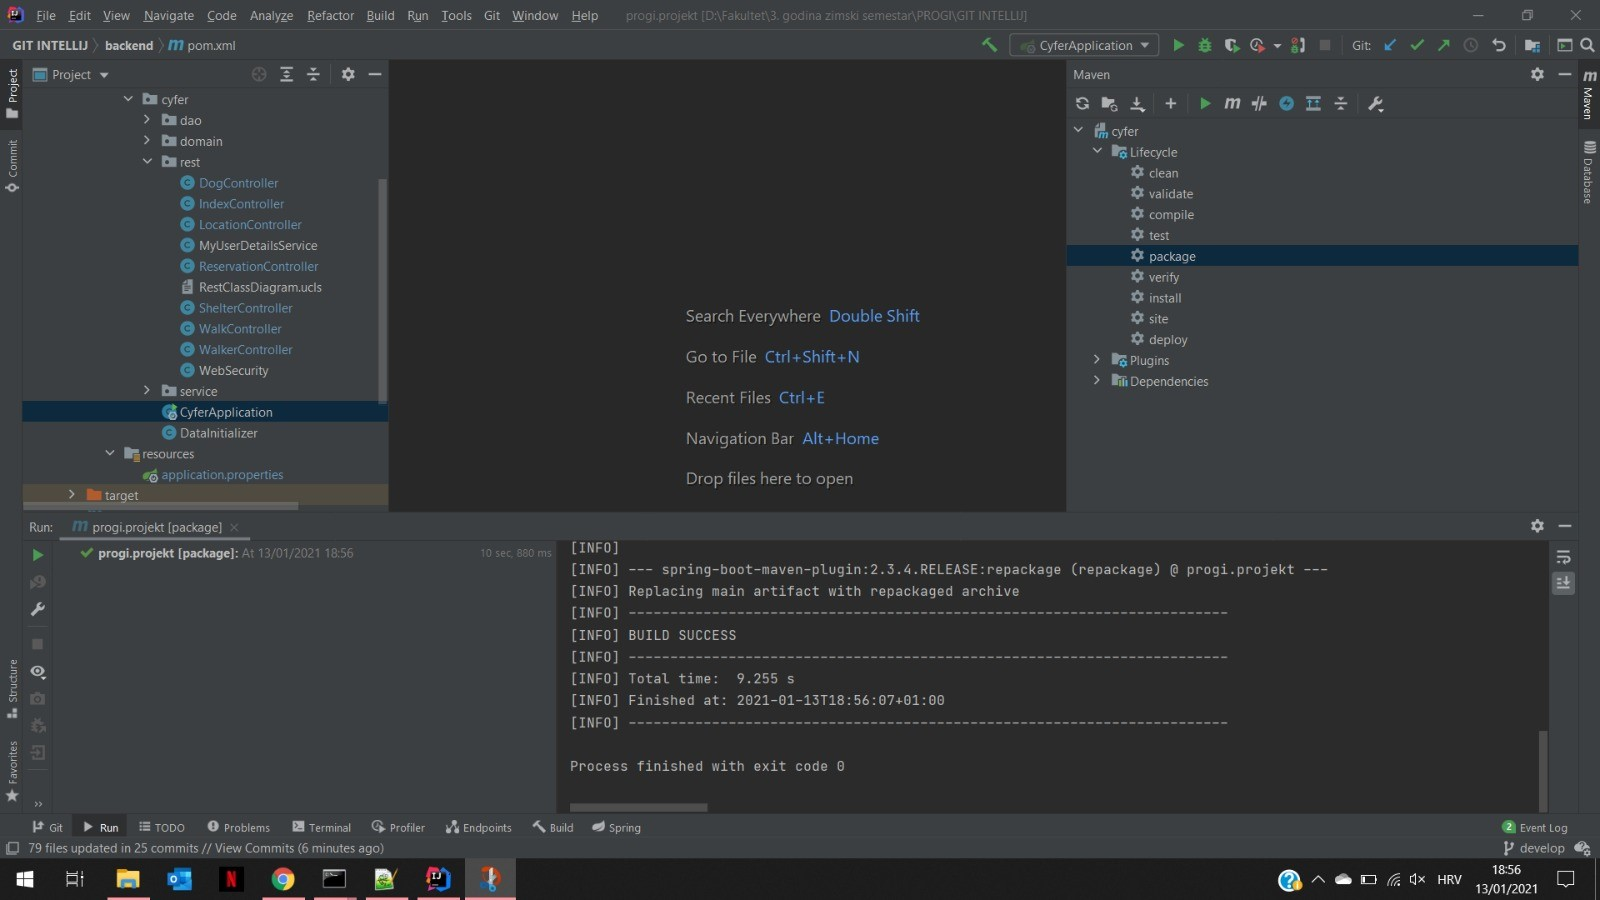
\includegraphics[scale=0.37]{slike/pustanje1.jpg}
			\caption{Generiranje .jar datoteke}
			\label{fig:pustanje1}
		 %veličina slike u odnosu na originalnu datoteku i pozicija slike
			\centering
		\end{figure}
		
		
		Kako bismo pustili u pogon našu backend aplikaciju, pozicionirali smo se u naredbenom retku u mapu backend u našem projektu i izvršili sljedeću naredbu:
		
		\centerline{
		\textbf{\textit{deploy:jar target/progi.projekt-1.0.jar --app cyfer-backend}}}
	
		~\\
		\noindent
		Backend aplikacija je nakon toga bila dostupna na internetu na URI-ju \textbf{\textit{\href{https://cyfer-backend.herokuapp.com}{https://cyfer-backend.herokuapp.com}}}. Grafičkog sučelja naravno nema, pa na sve zahtjeve koje šaljemo (samo putem URI-ja) dobivamo odgovore u obliku JSON-a.
		
		\subsection{Dodavanje baze podataka na Heroku}
		U fazi razvoja aplikacije koristili smo H2, dok smo na kraju izrade prešli na PostgreSQL bazu na localhostu. Kako bi baza bila dostupna nakon puštanja aplikacije u pogon, dodali smo ju na našu backend aplikaciju na Heroku kao add-on, te smo izmijenili aplication.properties kako bi bio omogućen pristup toj bazi. Da povezivanje bude moguće, morali smo stvoriti varijablu okruženja naredbom:
		\newline
		\\*
		\centerline{\textbf{
		\textit{heroku run echo \$JDBC\_DATABASE\_URL}}}
		
		\subsection{Puštanje u pogon frontend aplikacije}
		
		Deploy frontend aplikacije je nešto složeniji jer zahtjeva korištenje dockera i namiještanje proxyja. Naime, dok smo aplikaciju pokretali s localhosta u datoteci package.json imali smo definiran proxy (odnosno posrednik koji s frontenda preusmjerava HTTP zahtjeve na backend i vraća odgovor) koji je slušao na portu 8080 (defaultni port za spring boot backend aplikacije). Pri puštanju pogon morali smo dodati nekoliko novih datoteka koje će konfigurirati usmjeravanje tih zahtjeva, kao i sam prikaz grafičkog sučelja aplikacije definiranog na frontendu.
		Za virtualizaciju i prikaz smo koristili docker kojega smo konfigurirali u datoteci Dockerfile, a kao poslužitelj ngnix. Usmjeravanje putem proxyja smo konfigurirali novom datotekom default.conf unutar koje je zapisano da svi zahtjevi za backend trebaju imati prefiks /api, te smo taj prefiks dodali u kôd i na frontend i na backend kako bi mapiranje zahtjeva i vraćanje odgovora bilo funkcionalno.
		U Heroku smo stvorili aplikaciju cyfer-frontend. Pozicionirali smo se u frontend mapu našeg projekta i pokrenuli sljedeće naredbe iz naredbenog retka:\\
		
		\noindent
		\textbf{\textit{npm run build}}(izgradnja React aplikacije)\\
		\textbf{\textit{docker build -t registry.heroku.com/cyfer-frontend/web .}}(stvaranje slike)\\
		\textbf{\textit{docker push registry.heroku.com/cyfer-frontend/web}} („pushanje“ aplikacije na Heroku)\\
		\textbf{\textit{heroku container:release web --app cyfer-frontend }} (puštanje u pogon na dostupnom URL)\\
			
		\noindent	
		Aplikacija je nakon toga puštena u pogon i dostupna na:\\
		\textbf{\textit{\href{ https://cyfer-frontend.herokuapp.com}{https://cyfer-frontend.herokuapp.com}}}.
		
		\begin{figure}[H]
			\hspace*{-0.4in}
			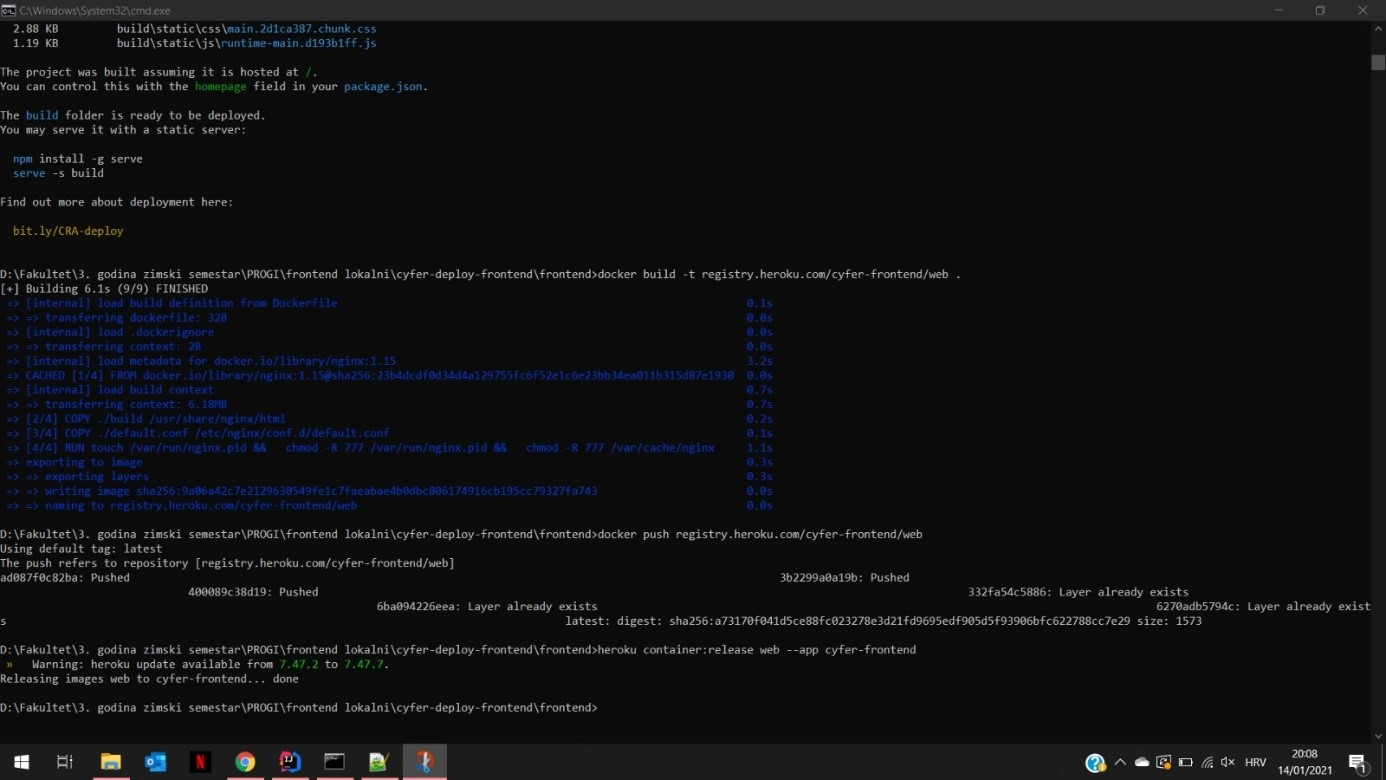
\includegraphics[scale=1.1]{slike/pustanje2.jpg}
			\caption{Pokretanje naredbi za deploy aplikacije}
			%veličina slike u odnosu na originalnu datoteku i pozicija slike
			\centering
		\end{figure}
	
		\begin{figure}[H]
			\hspace*{-0.54in}
			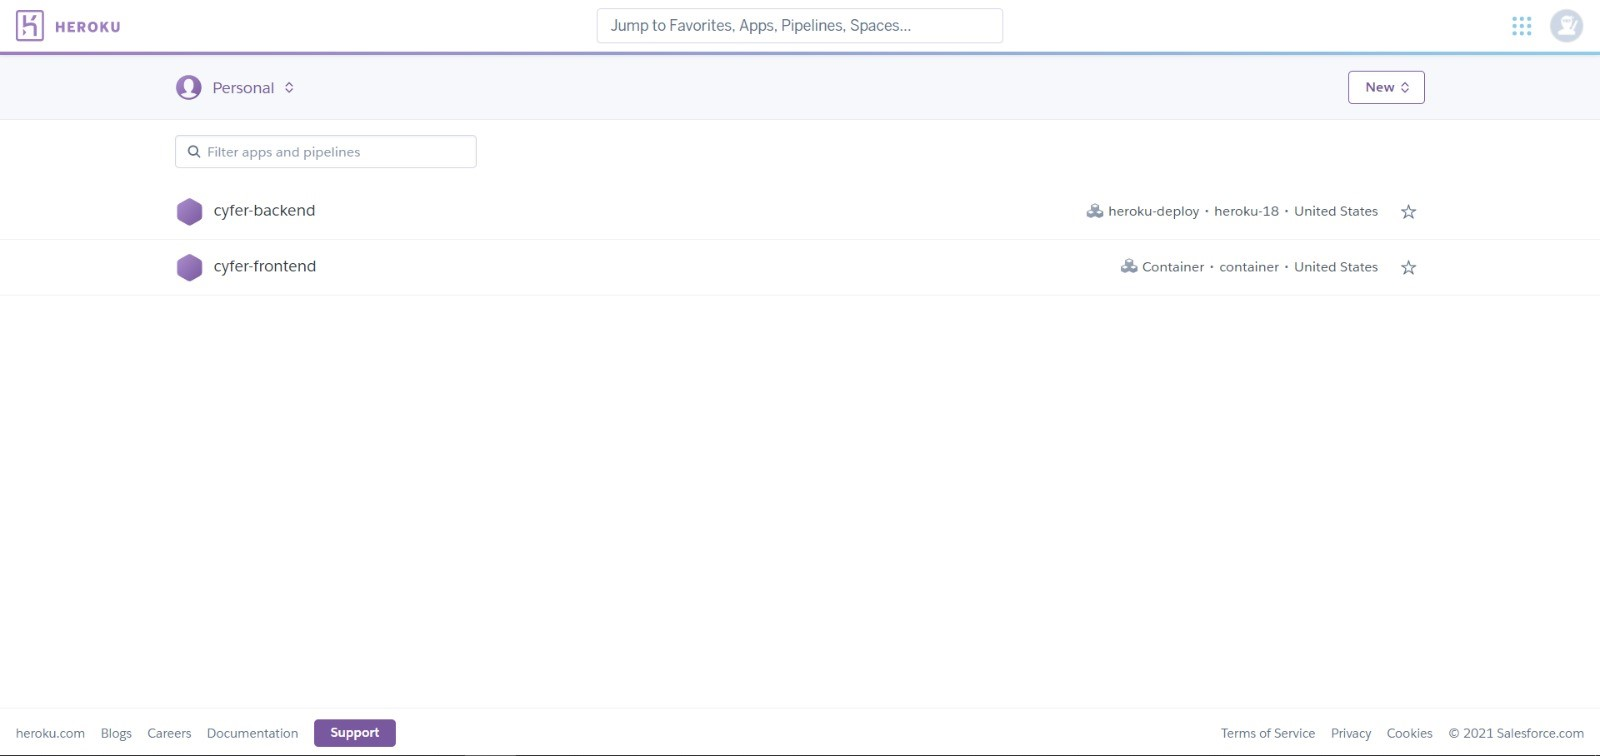
\includegraphics[scale=0.45]{slike/pustanje3.jpg}
			\caption{Deployani frontend i backend}
			%veličina slike u odnosu na originalnu datoteku i pozicija slike
			\centering
		\end{figure}
	
	
		
		
			\eject 